\documentclass[12pt]{elegantbook}

\definecolor{LightGray}{gray}{0.9}
\newcommand{\CN}{BIOS 7300\\[0.5cm] Survival Data Analysis}
\newcommand{\Ti}{Homework 4}
\newcommand{\Pf}{Dr. Tang}
\newcommand{\FN}{Zehao}
\newcommand{\LN}{Wang}
\usepackage[fontsize=14pt]{fontsize}

\usepackage{minted}

\usepackage{enumitem}
\renewcommand{\chaptername}{Homework}
\begin{document}
\begin{titlepage}
    \begin{center}    
    
\includegraphics[width=0.6\textwidth]{Tulane.png}\\[1cm]    
    
    \textsc{\Huge \CN}\\[0.5cm]
    \textsc{\large \Pf}\\[1.0cm]
    
    \textsc{\LARGE \Ti}\\[0.5cm]
    \textsc{\large \LN, \FN}\\
    {Master student in Statistics of Math Dept.}
    
    % Author and supervisor
    
    \vfill
    
    % Bottom of the page
    {\Large \emph{\today}}
    
    \end{center}
\end{titlepage}

\thispagestyle{empty}
\tableofcontents
\setcounter{chapter}{3}
\chapter{}

    
    \begin{exercise*}[1]
        In a survival analysis we are interested in studying if the treatment effects may be affected by gender. A proportional hazards model is fitted with treatment ($=1$ the for new treatment and $=0$ for the standard treatment) and gender ($=0$ for females and $=1$ for males) as covariates, including the interaction. Reference coding with the level $0$ as the reference level is applied to both factors. The parameter estimates are given in the following table: 
        \begin{table}[H]
            \centering
            \begin{tabular}{lrr}
            \hline
            Parameter                 & Estimate & Standard Error \\ \hline
            Gender                    & 0.04328  & 0.12988        \\
            Treatment                 & -6.66091 & 0.73266        \\
            Gender $\times$ Treatment & 0.79568  & 0.82733        \\ \hline
            \end{tabular}
        \end{table}
        \begin{enumerate}[(a)]
            \item Compute treatment effect for both genders, i.e., the hazards ratio of the new treatment vs the standard treatment for females and males. 
            \item Compute the interaction effect, the ratio of the hazards ratio of the new treatment vs the standard treatment among females and hazards ratio of the new treatment and the standard treatment among males.\label{q1_pb}
            \item Compute the $95\%$ confidence interval for the interaction effect you computed in part~\ref{q1_pb} and test if the interaction is significant. 
        \end{enumerate}
    \end{exercise*}

    \begin{solution}
        \begin{enumerate}[(a)]
            \item Let $X_1$ be treatment, and $X_2$ be gender. So, the Cox Proportional Hazard model is: 
            \[h(t, X, \beta)=h_0(t)\exp(\beta_1X_1+\beta_2X_2+\beta_3X_1X_2)\]
            And $\beta_1=-6.66091$, $\beta_2=0.04328$, $\beta_3=0.79568$. 

            For female, $X_2=0$, 
            \[h(t, X, \beta)=h_0(t)\exp(-6.66091X_1)\]
            \[HR(t, X_1=1\text{ V.S. }X_1=0)=\frac{\exp(-6.66091)}{1}\approx 0.00127998. \]
            For male, $X_2=1$, 
            \[h(t, X, \beta)=h_0(t)\exp(-6.66091X_1+0.04328+0.79568X_1)\]
            \[HR(t, X_1=1\text{ V.S. }X_1=0)=\frac{e^{-6.66091+0.04328+0.79568}}{\exp(0.04328)}\approx 0.00283637. \]
            \item \[HR(X_1=1\text{ V.S. }X_1=0, X_2=0)=0.00127998 \]
            \[HR(X_1=1\text{ V.S. }X_1=0, X_2=1)=0.00283637 \]
            \[\frac{HR(X_1=1\text{ V.S. }X_1=0, X_2=0)}{HR(X_1=1\text{ V.S. }X_1=0, X_2=1)}\approx 0.45127. \]
            \item \[0.45127+ \chi_{0.975}(1)\times se(\hat{\beta})=0.45127+5.024\times0.37334921=2.327.\]
            \[0.45127- \chi_{0.025}(1)\times se(\hat{\beta})=0.45127-0.001\times0.37334921=0.4509. \]
            \[\left(\frac{0.45127}{0.3733}\right)^2=1.4613. \]
            \[p\text{-}value=0.2267234>0.05. \]
            So, it is not significant. 
        \end{enumerate}
    \end{solution}

    \begin{exercise*}[2]
        In a liver transplant study (data set “Survival of liver transplant recipients.dat”), we are interested in studying how age (“age”: patient ages measured in years) and disease severity (“disease”: three levels in disease, 1, 2, and 3) are related with the survival time. We treat “age” as a variate and “disease” as a categorical variable, and apply a proportional hazard model with additive effects from age and disease. Please write down the proportional hazard model (you need to explicitly define the variables about the disease severity according to your coding system) and complete the following based on the model. Note that the variable “time” contains the survival times and “status” is the indicator for death; a value of 0 in “status” indicates that the survival time is right censored. 
        \begin{enumerate}[(a)]
            \item Estimate the parameters using a statistical software package.
            \item Interpret the coefficient of age. Is age a significant predictor for the survival outcome based on the model?
            \item If age is measured in months, what value would the coefficient of age be? Is age a significant predictor for the survival outcome based on the model using the new scale?
            \item Interpret the coefficients of the disease severity. Are there significant difference in the survival outcomes among the different groups with different disease severity?
        \end{enumerate}
    \end{exercise*}

    \begin{solution}
        \[h(t)=h_0(t)\exp(\alpha X_{age}+\beta X_{disease_2}+\gamma X_{disease_3})\]
        \begin{enumerate}[(a)]
            \item \begin{minted}[frame=lines,
                framesep=2mm,
                baselinestretch=1.2,
                bgcolor=LightGray,
                fontsize=\footnotesize]{SAS}
DATA HW4;
INFILE "Z:\Documents\GitHub\MS-Stat-Tulane
\Survival Data Analysis\HW04
\Survival of liver transplant recipients.dat" FIRSTOBS=2;
INPUT patient age gender disease time status cof; 
PROC PHREG DATA=HW4;
CLASS disease (ref=first);
MODEL time*status(0) = age disease;
HAZARDRATIO disease / AT () DIFF=ALL;
RUN;
            \end{minted}
            \begin{figure}[H]
                \centering
                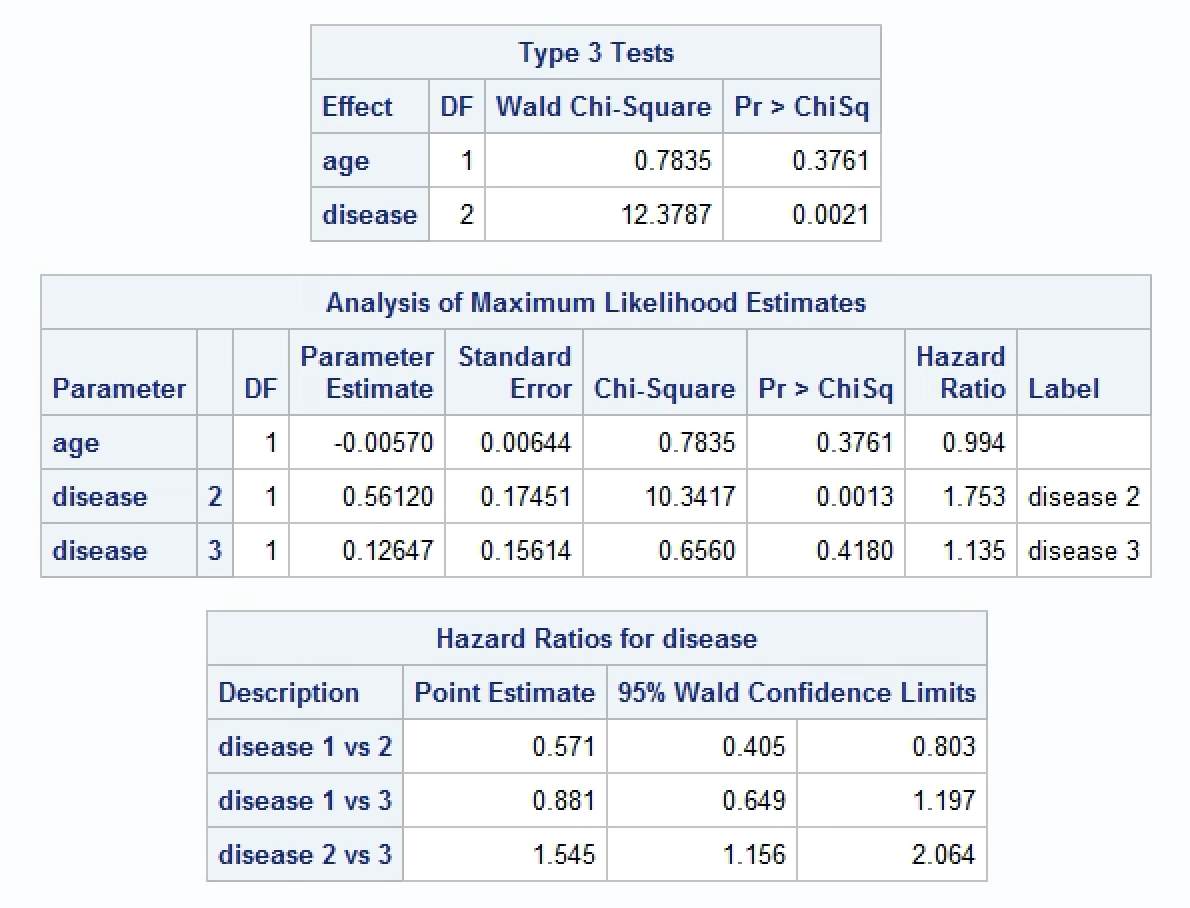
\includegraphics[width=0.8\textwidth]{HW4_1.png}
            \end{figure}
            \item The coefficient of age is $-0.0057$. It means that for every one year increase in age, the hazard ratio will decrease by multiply $e^{-0.0057}=0.9943$. And it is not significant. 
            \item $age'=12*age$, So, the new estimated coefficient is $-0.0057/12$, and std error is $0.00644/12$. P-value is invariant. It is not significant.
            \item For every one year increase, hazard ratio of the disease 2 will increase by multiply $e^{0.56120}=1.75$ compared to without disease 2. And hazard ratio of the disease 3 will increase by multiply $e^{0.12647}=1.13$ compared to without disease 3. 
            
            And the difference between disease 2 and without disease 2 is significant. 
        \end{enumerate}
    \end{solution}

    \begin{exercise*}[3]
        Use the data in the last question and continue to use age and disease severity as predictors. Now we would like to test if there are interactions between age and disease severity. Please write down the proportional hazard model and answer the following questions based on the model. 
        \begin{enumerate}[(a)]
            \item Interpret the coefficients of the interaction terms. 
            \item Interpret the coefficient of age.
            \item Are there significant interactions between age and disease severity?
        \end{enumerate}
    \end{exercise*}

    \begin{solution}
        \[h(t)=h_0(t)\exp(\alpha X_{age}+\beta_1 X_{disease_2}+\beta_2 X_{disease_3}+\gamma_1X_{age}X_{disease_2}+\gamma_2X_{age}X_{disease_3})\]
    \end{solution}
    \begin{minted}[frame=lines,
        framesep=2mm,
        baselinestretch=1.2,
        bgcolor=LightGray,
        fontsize=\footnotesize]{SAS}
PROC PHREG DATA=HW4;
CLASS disease (ref=first);
MODEL time*status(0) = age|disease;
HAZARDRATIO disease /at () DIFF=ALL;
RUN;
    \end{minted}
    \begin{figure}[H]
        \centering
        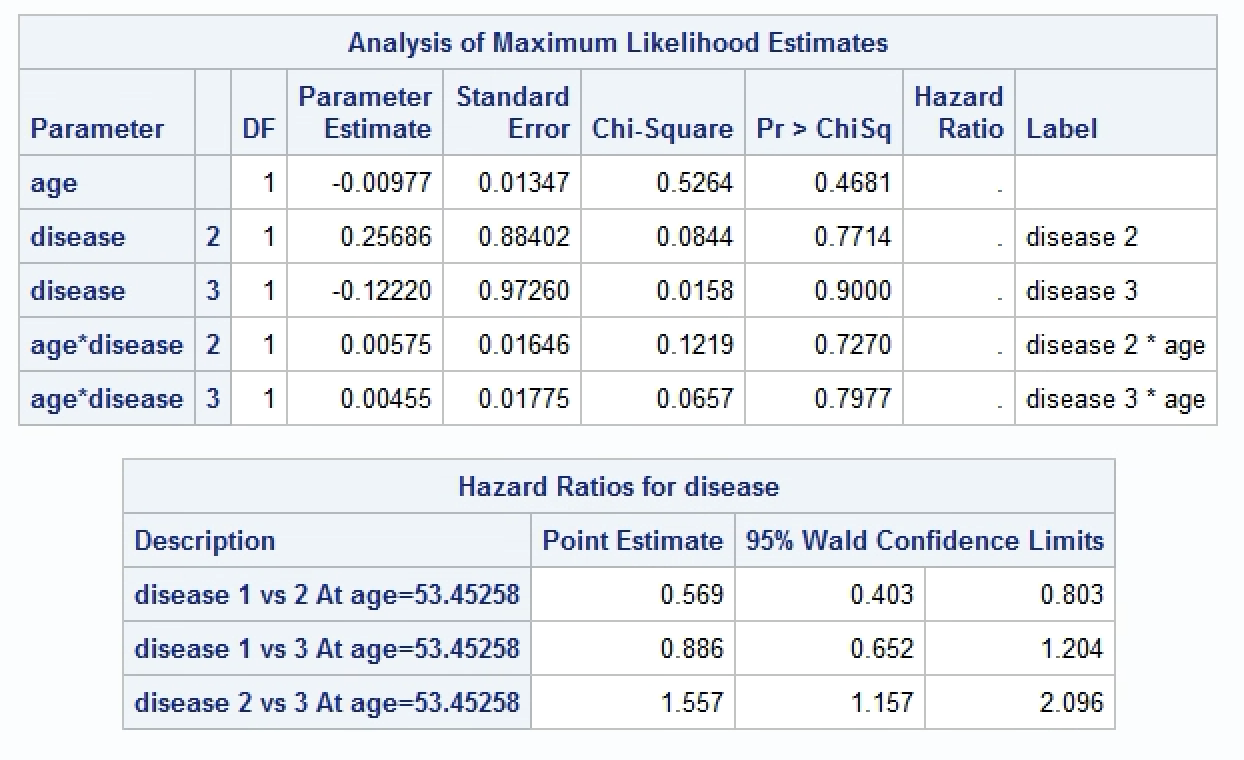
\includegraphics[width=0.8\textwidth]{HW4_2.png}
    \end{figure}
    \begin{enumerate}[(a)]
        \item For $\gamma_1$, it means Log-HR will increase $0.00575$ when the interaction of age and disease 2 increase one unit. 
        
        For $\gamma_2$, it means Log-HR will increase $0.00455$ when the interaction of age and disease 3 increase one unit. 
        \item For $\alpha$, it means Log-HR will decrease $0.00977$ when the age increase one unit. 
        \item None of them are significant. Because the p-value of them are larger than $0.05$.
    \end{enumerate}
    
\end{document}